\section{Problem Formulation}

Cyclic pursuit is a distributed algorithm for achieving circular formations. In particular, we assume each agent knows its own state and that of the preceding agent in the formation. In order to achieve a circle the network must be strongly connected and therefore the corresponding graph for the network is the stated ring di-graph. The algorithm is based on continuous time dynamics and controls.

In order to describe the formation achieved we start by describing the dynamics of the system. Each individual agent is described as a non-holonomic particle with a common constant velocity that can be steered using the input. Its dynamics with respect to an some reference frame are
\begin{align}
\dot{x}_i &= v \cos \psi_i \\
\dot{y}_i &= v \sin \psi_i \\
\dot{\psi}_i &= u_i  
\end{align}

$\vec{r}_i=(x_i,y_i)$ represent the Cartesian coordinates on the euclidean plane for the position of agent $i$. $v$ is a constant velocity, common for all agents, and $\psi_i$ the heading of the velocity which can be modified by means of the control input $u_i$.

Each agent $i$ knows its own state in a local reference frame. It is also able to measure the relative position of the preceding agent $j= \textrm{mod}(i+1,n)$ and heading of its velocity with respect to some local reference frame. All the information about the agent $j$ can be achieved without any communication between the agents by relative position measurements. This feature is highly desirable and we will try to preserve by all means.

The relative position vector $\vec{r}_{ij} = \vec{r}_j - \vec{r}_i$ is expressed in a local coordinate frame by its module $\rho_{ij}$ and relative its argument $\kappa_{ij}$ with respect to the velocity heading $\psi_i$. The relative argument between the heading of the velocity preceding agent $j$ $\psi_j$ and the $\vec{r}_{ij}$ vector is defined as $\theta_{ji}$. These two parameters are determined by the relative position measurement.
\begin{figure}[h]
	\centering
	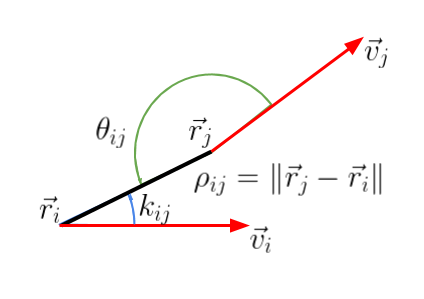
\includegraphics[height=1.7in]{Attachments/Geometry.png}
	\caption{Description of the geometry between agent $i$ and $j$.}
	\label{fig:Geometry}
\end{figure}

Cyclic pursuit attempts to keep this relative bearing $k_{ij}$ constant and equal to the reference $\alpha_i^*$. $^*$ all along this report will mean that some value is constant and predetermined. $\mu$ is a positive gain that controls the control action proportional to the difference between the actual relative bearing $\kappa_{ij}$ and the reference $\alpha_i$. The control law used to achieve this is given in \cite{galloway2013symmetry}
\begin{equation}
  u_i = \mu  \sin(\kappa_{ij} -\alpha_i^*) + \frac{1}{\rho_{ij}} ( \sin \kappa_{ij} + \sin \theta_{ji})
\end{equation}

The control law is the addition of two terms. The first term is a proportional-like term that intends to make the actual relative bearing $\kappa_{ij}$ converge to the desired relative bearing $\alpha_i^*$. The second term attempts to compensate for the angular motion between the two agents. This is done by computing the lateral velocity between $i$ and $j$ as the projection of the velocities of $i$ and $j$ along the relative position vector. This lateral velocity is converted into angular rate using the inter-agent distance $\rho_{ij}$.

This control law is shown to guarantee to converge to some formation in \cite{galloway2013symmetry} where the convergence is shown by showing the asymptotic stability of the network to some formation manifold. 
If all the agents have an equal constant velocity the shape of the formation is determined by $\alpha^* = [\alpha_1^* \quad \alpha_2^* \quad \ldots \quad \alpha_n^*]^T$ for agents $\ i\in\{1,2, \ldots, n\}$ as shown in \cite{galloway2013symmetry}. Furthermore, it shown that to achieve circular formations it is necessary that all $\alpha_i^*$ have the same sign. Without loss of generality, we consider only positive $\alpha_i^*$ from here on. 

Under those conditions, the same reference states Cylic Pursuit will converge into a converging/diverging spiral, and under certain conditions it will converge into a circle. The condition for the circular formation with no overlap is
\begin{equation}
  \alpha^{*T} \mathbb{1} = \pi
\end{equation}

The simplest formation satisfying the previous conditions achieves the regular n-sided polygon by using $\alpha_i = \pi / n$. We can see that under this conditions, and for $n=4$ the circular formation in the introduction is achieved.
\begin{figure}[h]
	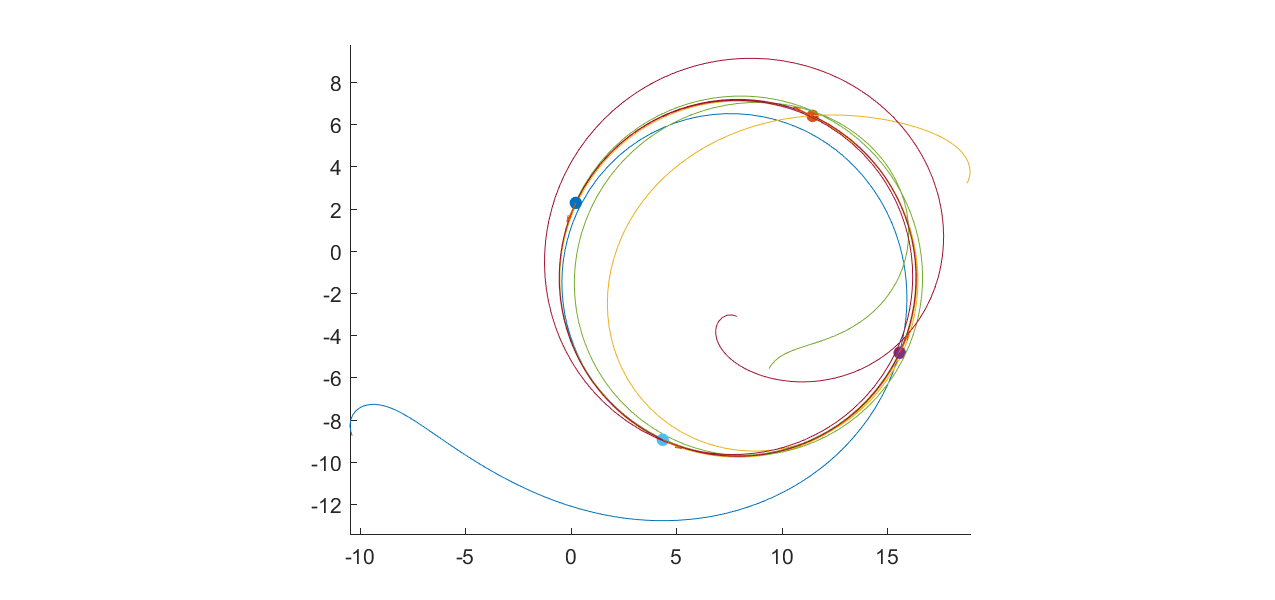
\includegraphics[width=\linewidth]{Attachments/Figure21.png}
	\caption{Cyclic Pursuit convergence to a circle.}
	\label{fig:CircleConvergence}
\end{figure}

Besides, the conditions for convergence (divergence) from the center are $\alpha^{*T} \mathbb{1} > \pi ( < \pi)$, then the spiral will diverge (converge). This fact will be leveraged in the upcoming sections.

While this algorithm is interesting from a theoretical point of view it has two main disadvantages that prevent its application

\paragraph{Radius stability}
The stability of the algorithm relies completely on angular criteria on the circle. These criteria are independent of the radius implying there is no control on the radius and size of the formation nor stability under perturbations.

Another issue is the difficulty to predict the parameters of the final formation given the initial conditions. No prediction on the size of the formation (even if no perturbations are present) can be obtained by inspection of the initial conditions.

\paragraph{Network robustness}
The convergence of the algorithm to a circle relies on achieving the $\alpha^{*T} \mathbb{1} = \pi$ criterion. This implies the need of coordination and that if an agent leaves or joins the formation will no longer work. Typically, adding a new agent will increase the sum of the elements of $\alpha^{*T} \mathbb{1}$ and removing an agent will reduce it. The algorithm is not robust from a network variation point of view.

A solution to the radius stability is provided in \cite{ramirez2010distributed}. This solution however, is dependent on the $\alpha^{*T} \mathbb{1} = \pi$ condition and therefore is not considered to be robust to changes in the network. In order to provide a better understanding of the solution we will first give a more insightful description of the two issues that will be addressed in this project.



